% !TeX root = ../tesis.tex


\chapter{Eritrocitos y sus patologías}
En este capítulo


\section{Morfología y enfermedades}
\label{section:results}


La sangre humana está compuesta principalmente por eritrocitos o glóbulos rojos (RBCs por sus siglas en inglés), leucocitos, plaquetas y plasma sanguíneo \cite{mescherJunqueirasBasicHistology2024}. El plasma constituye el medio continuo en el que se encuentran suspendidos todos estos elementos y está formado por agua, electrolitos, proteínas plasmáticas, carbohidratos, lípidos y vesículas extracelulares \cite{mescherJunqueirasBasicHistology2024}.

\noindent En el rango espectral de 250 a 1100 nm, los eritrocitos son los principales responsables de la absorción y el esparcimiento óptico de la sangre: su contribución puede superar hasta por tres órdenes de magnitud la de los demás componentes \cite{bosschaartLiteratureReviewNovel2014a}. Esta diferencia se debe al contraste entre su índice de refracción y el del plasma. Por ello, para describir la interacción luz–sangre, en este trabajo se consideran únicamente a los eritrocitos y al plasma: el primero actúa como la partícula esparcidora  y el segundo como el medio circundante.

 \noindent El plasma sanguíneo es una solución acusosa compuesta por proteínas, nutrientes, electrolitos, entre otros. Aún cuando presenta absorción y esparcimiento, originados principalmente por sus proteínas (como albúmina y fibrinógeno) y por las plaquetas, contribuye en menor medida a la respuesta óptica global dentro del rango de 250 a 1100 nm. No obstante, en ciertas condiciones patológicas su absorción puede incrementarse \cite{bosschaartLiteratureReviewNovel2014a}.
 
\noindent Los eritrocitos, por su parte, son células terminalmente diferenciadas\footnote{Una célula terminalmente diferenciada se define como aquella que, al adquirir funciones especializadas, pierde
	su capacidad de proliferar de manera irreversible. Por ejemplo, los eritrocitos y queratinocitos de los mamíferos,
	sufren una detención irreversible de su crecimiento al perder su núcleo durante la diferenciación terminal \cite{saccoCellCycleReactivation2002}.} que carecen de núcleo y están constituidas casi por completo de hemoglobina, la proteína responsable de sus características de absorción óptica \cite{bosschaartLiteratureReviewNovel2014a}. A su vez, la hemoglobina presenta firmas espectrales definidas en el rango entre 250–1100 nm, las cuales dependen de su estado químico —principalmente oxihemoglobina ($\text{HbO}_2$) y desoxihemoglobina (Hb)— \cite{bosschaartLiteratureReviewNovel2014a}. A través de la hemoglobina, los eritrocitos desempeñan su función fisiológica fundamental de transporte de oxígeno \cite{palTextbookMedicalPhysiology2021}.


\noindent La eficiencia en el transporte de oxígeno está estrechamente vinculada con la geometría de los eritrocitos. Estas células poseen una membrana sostenida por un citoesqueleto altamente flexible que les confiere su morfología característica \cite{palTextbookMedicalPhysiology2021}, observable en la micrografía electrónica de barrido (SEM por sus siglas en inglés) mostrada en la Fig.~\ref{subfig:SEM}, tomada de \cite{alummoottilScanningElectronAtomic2023}. Como se observa en el diagrama de un corte axial de un eritrocito en la Fig.~\ref{subfig:ery}, los eritrocitos presentan un contorno ovalado y un diámetro promedio de aproximadamente 7.5~$\mu$m. Su forma incluye una depresión central que reduce el espesor en la región media, dando lugar a un disco bicóncavo con un grosor aproximado de 2.6~$\mu$m en los bordes y 0.75~$\mu$m en el centro \cite{palTextbookMedicalPhysiology2021}. Esta geometría no solo es fundamental para su función fisiológica, al proporcionar una alta relación superficie-volumen y facilitar el intercambio de gases \cite{palTextbookMedicalPhysiology2021}, sino que también influye directamente en su comportamiento óptico y en la manera en que esparcen la luz \cite{bosschaartLiteratureReviewNovel2014a}.




\begin{figure}[t]
	\centering
	\sidesubfloat[First image]{
	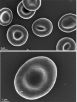
\includegraphics[width=0.3\textwidth]{../Figuras/SEM_erythrocyte.pdf}\label{subfig:SEM}}\hspace{0.5cm}
	\sidesubfloat[Second image]{	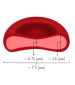
\includegraphics[width=0.35\textwidth]{../Figuras/erythrocyte.pdf}\label{subfig:ery}}
	\caption{Estructura de un eritrocito sano. \textbf{a)} Micrografías SEM de eritrocitos de pacientes sanos. La micrografía superior muestra eritrocitos de forma bicóncava normal con interacción limitada, mientras que la inferior muestra un eritrocito sano con una membrana ligeramente granular; imágenes extraídas y adaptadas de \cite{alummoottilScanningElectronAtomic2023}. \textbf{b)} Diagrama de un corte longitudinal de un eritrocito que muestra las dimensiones de la célula. }
	\label{fig:erythrocytes}
\end{figure}


\begin{figure}[t]
	\centering
	\sidesubfloat[First image]{
		
\includegraphics[width=0.3\textwidth]{../Figuras/erythrocyte_health.pdf}\label{subfig:SEM}}\hspace{0.5cm}
	\sidesubfloat[Second image]{	
\includegraphics[width=0.22\textwidth]{../Figuras/spherocytosis.pdf}\label{subfig:ery}}
	
	\vspace{0.5cm}
	
	\sidesubfloat[Second image]{	
\includegraphics[width=0.31\textwidth]{../Figuras/microcyte.pdf}\label{subfig:ery}}
	\sidesubfloat[Second image]{	
\includegraphics[width=0.31\textwidth]{../Figuras/macrocyte.pdf}\label{subfig:ery}}
	
		\vspace{0.5cm}
		
	\sidesubfloat[Second image]{	
\includegraphics[width=0.8\textwidth]{../Figuras/sickle_cell.pdf}\label{subfig:ery}}	
	
	\caption{Estructura de un eritrocito sano. \textbf{a)} Micrografías SEM de eritrocitos de pacientes sanos. La micrografía superior muestra eritrocitos de forma bicóncava normal con interacción limitada, mientras que la inferior muestra un eritrocito sano con una membrana ligeramente granular; imágenes extraídas y adaptadas de \cite{alummoottilScanningElectronAtomic2023}. \textbf{b)} Diagrama de un corte longitudinal de un eritrocito que muestra las dimensiones de la célula. }
	\label{fig:erythrocytes}
\end{figure}


Due to various diseases, RBCs can be deformed in terms of size and shape. For example, an RBC is identified25 as a macrocyte if its diameter is larger than 8.5 m, even though it
may have a biconcave shape like an ordinary RBC. Similarly,
an RBC with a diameter smaller than 7.0 m is identified as
a microcyte.25 Among various types of shape-deformed
RBCs, sickle cells are identified by their extraordinary thin
and long structures with pointed ends,26 whereas spherocytes
have almost spherical geometries.27
Microcytosis and macrocytosis have clinical significance
because they may indicate other serious underlying diseases.
Microcytosis is observed mainly in disorders in iron metabolism or deficiencies in hemoglobin synthesis,28 whereas macrocytosis is mostly observed in drug use, alcoholism, liver
diseases, myeloma, and leukemia.29 On the other hand, sickle
cells are encountered in sickle-cell anemia or sickle-cell trait,
which are caused by abnormal hemoglobin structures. Due to
their extraordinary shape, sickle cells may not be able to pass
through capillaries, blocking the blood flow.30,31 In the case of
the sickle-cell anemia, 30 to 60% of RBCs may have sickle
shapes, whereas this ratio drops to only 1% for the sickle-cell
trait.26 In general, the number of sickle cells depends on various factors, particularly deoxygenation levels.26,30 Finally,
spherocytes are commonly observed in hereditary spherocytosis disease, which further leads to anemia, splenomegaly,
jaundice, and many other clinical symptoms.32
Currently, most automated diagnosis setups rely on mean
corpuscular volume MCV to detect the deformation of
RBCs in terms of size. Specifically, high and low MCV values
may indicate the presence of macrocytes and microcytes, respectively. However, MCV measurements are usually insufficient for a reliable diagnosis, and peripheral blood smears are
required, especially in the early stages of macrocytosis.29 As
opposed to microcytes and macrocytes, sickle cells can be
diagnosed via biochemical and genetic tests, which are available only in specialized laboratories,25,33 and spherocytes are
usually detected via mean corpuscular hemoglobin concentration and RBC width measurements.32 Nevertheless, blood
smear tests remain as the gold standard of diagnosing sickle
cells and spherocytes, as for microcytes and macrocytes.
As presented in this paper, ordinary and deformed RBCs,
i.e., microcytes, macrocytes, sickle cells, and spherocytes, can
be distinguished from each other using a complete analysis of
SCS values. Based on our results, we offer a fast and reliable
technique to detect deformed RBCs in a blood sample using
an automated diagnosis setup

